\chapter{Introduction} 
\lhead{Chapter 1. \emph{Introduction}}
\label{chap.1}

\section{Motivation}

The widespread deployment of quantum computing threatens the security of current encryption systems that protect file transfer protocols. Shor's algorithm, when executed on a sufficiently powerful quantum computer, can factor large integers and compute discrete logarithms in polynomial time — breaking RSA, DSA, and Elliptic-Curve Diffie-Hellman (ECDH) \cite{shor1994algorithms}. Grover's algorithm provides a quadratic speedup for symmetric key search, effectively halving the security level of symmetric ciphers \cite{grover1996fast}.

Of particular concern is the \textit{``Harvest Now, Decrypt Later''} (HNDL) threat model, where adversaries capture encrypted network traffic today for decryption once quantum computers become available \cite{mosca2018cybersecurity}. This threat demands proactive migration to quantum-resistant alternatives, especially for systems handling sensitive data transfers.

The motivation for this project is to counter this threat by designing a complete, production-grade secure file transfer protocol that provides confidentiality, integrity, and authentication guarantees even against adversaries possessing quantum computers.

\section{Problem Statement}

Current Secure File Transfer Protocols (SFTP) rely on classical encryption algorithms such as RSA and Elliptic Curve Cryptography (ECC). Although these algorithms are secure against classical computers, they are vulnerable to quantum algorithms:

\begin{itemize}
    \item \textbf{Shor's Algorithm:} Breaks the integer factorization (RSA) and discrete logarithm (ECC/DH) problems in polynomial time.
    \item \textbf{Grover's Algorithm:} Reduces the effective security of symmetric key algorithms by half (e.g., AES-128 becomes effectively 64-bit against quantum search).
\end{itemize}

\noindent\textbf{Issue:} Current file transfer systems lack quantum-resistant cryptographic mechanisms.\\
\textbf{Impact:} Organizations and individuals relying on secure data transfer face long-term confidentiality risks.\\
\textbf{Goal:} To design, implement, and deploy a post-quantum secure file transfer protocol using NIST-standardized algorithms with production-grade features.

\section{Threat Model}
Fig.~\ref{fig:threat} illustrates the threat modeling for Quantum Secure File Transfer Protocol (Q-SFTP). The threat model considers the following adversary capabilities:

\begin{itemize}
    \item Passive eavesdropping on all network traffic (HNDL threat).
    \item Active man-in-the-middle (MITM) attacks attempting to intercept or modify handshake messages.
    \item Replay attacks using captured legitimate messages.
    \item File tampering during transit or at rest on the server.
    \item Malicious file uploads (executables, spoofed extensions).
    \item Unauthorized access through credential theft or privilege escalation.
\end{itemize}

\begin{figure}[!hbt]
    \centering
    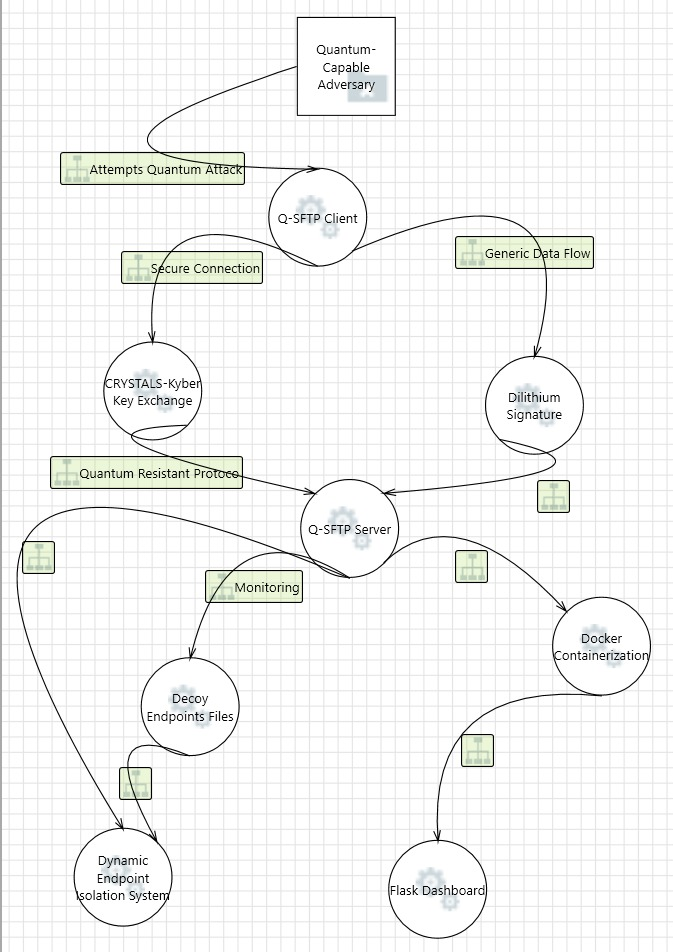
\includegraphics[width=0.88\textwidth]{Figures/threat_model.jpg}
    \caption{Threat Model of Quantum Secure FTP}
    \label{fig:threat}
\end{figure}

\section{Goals}

The main objectives of this project are:
\begin{enumerate}
    \item To design and implement a \textbf{four-phase PQC handshake protocol} using CRYSTALS-Kyber512 for key encapsulation and CRYSTALS-Dilithium2 for digital signatures, achieving mutual authentication and ephemeral session key derivation.
    
    \item To implement \textbf{BLAKE2b-256 file integrity verification} with dual-side hash comparison, a persistent hash registry, and periodic background integrity monitoring.
    
    \item To develop a \textbf{chunked resumable transfer protocol} with persistent state tracking, enabling reliable file transfer over unreliable network conditions.
    
    \item To enforce \textbf{role-based access control (RBAC)} with three tiers (Administrator, Standard, Guest) and per-user directory isolation.
    
    \item To provide \textbf{automatic metadata stripping} for privacy preservation and \textbf{malicious file protection} via extension blacklisting and magic number validation.
    
    \item To deploy the system as a \textbf{modern web application} with a browser-based GUI that abstracts all cryptographic complexity behind an intuitive interface.
\end{enumerate}


\section{Research Methodology}

The research is guided by the following questions:
\begin{enumerate}
    \item What are the vulnerabilities of contemporary SFTP protocols against quantum computing threats, and how does the ``Harvest Now, Decrypt Later'' model exacerbate these risks?
    
    \item How can NIST-standardized post-quantum cryptographic algorithms (CRYSTALS-Kyber and CRYSTALS-Dilithium) be integrated into a practical, deployable file transfer protocol?
    
    \item What additional security layers (file integrity, access control, metadata stripping, malicious file protection) are necessary for a production-grade post-quantum file transfer system?
    
    \item How does the performance of a PQC-based file transfer protocol compare to classical SFTP in terms of handshake latency, transfer throughput, and cryptographic overhead?
\end{enumerate}

\section{Structure of the Project}

The rest of the project is presented in the following chapters:

\begin{itemize}
    \item Chapter~\ref{chap.2} presents the preliminary background and related work: basics of secure file transfer, quantum-safe cryptography, and the Q-TLS handshake model.
    
    \item Chapter~\ref{chap.3} presents the results of the literature survey, comparing existing approaches, describing their limitations, and identifying the research gaps that motivated this project.
    
    \item Chapter~\ref{chap.4} presents the proposed system in detail: four-tier architecture, PQC handshake protocol (with formal mathematical notation), BLAKE2b integrity system, resumable chunked transfer protocol, file validation, metadata stripping, RBAC, activity logging, web GUI, admin panel, and deployment options.
    
    \item Chapter~\ref{chap.5} describes the key contributions, including a defense-in-depth analysis, novel findings during development, and a feature comparison with existing solutions.
    
    \item Chapter~\ref{chap.6} presents the experimental results: handshake verification, security testing, transfer performance evaluation, and comprehensive security analysis.
    
    \item Chapter~\ref{chap.7} concludes the project by summarizing achievements and discussing limitations.
    
    \item Chapter~\ref{chap.8} outlines future work including hybrid key exchange, formal verification, and WebSocket transport.
\end{itemize}
